
\section{Study Area}
% Provide a description of the sampling methods, field area, and geology.
% - Include maps or figures if necessary.

% want table with catchment characteristics
% also remember to include a table with abbreviations


The Melamchi-Indrawati catchment (85.441 - 85.601 E, 27.822 - 28.157 N) study area ranges from 790 to 5700 m a.s.l. (metres above sea level). The Melamchi River is a tributary of the larger Indrawati River and runs through the catchment draining an area of 325km${^2}$. The catchment is has a mean slope of 20\% and a mean elevation of 2400m (see Figure \ref{fig:map}). 

\subsection{Geological Setting}

% Need to add Himalayan background

The overall geology is largely comprised of silicate metamorphic rock. The geology of Melamchi is characterised by banded gneiss, feldspathic schist and laminated quartzite of the Higher Himalayan Crystalline Sequence (HHCS) (\textcite{dhitalGeologyNepalHimalaya2015}; see Figure \ref{fig:map}). To the south of the confluence of the Melamchi River to its parent Indrawati river lies the Main Central Thrust (MCT) which separates the HHCS from the Lower Himalayan Sequence (LHS) (\cite{dhitalGeologyNepalHimalaya2015}; \cite{grafGeomorphologicalHydrologicalControls2023}).


% \begin{table}[h!]
%     \centering
%     \begin{small}
%     \begin{tabular}{p{3cm} p{1cm} p{1cm} p{1.8cm} p{1.9cm} p{1.5cm} p{3cm}}
%            \hline
%            \textbf{Catchment} & \textbf{Area} & \textbf{Mean Slope} & \textbf{Mean Elevation} & \textbf{Elevation Range} & \textbf{Geology} & \textbf{Location Range (DD)} \\[4pt]
%                               & (km$^2$)    & (\%)                & (m)                     & (m)                      &                &  \\[4pt]
%            \hline
%            Melamchi Khola     & 325         & 20                  & 2400                    & 786--5697                & HHCS           & 85.441--85.601 \phantom{i}E  27.822--28.157 \phantom{i}N \\[4pt]
%            \hline
%     \end{tabular}
%     \end{small}
%     \caption{Melamchi catchment characteristics. Area, Slope, Elevation data taken from \cite{asterGlobalDigitalElevation2018}. Geology adapted from \cite{dhitalGeologyNepalHimalaya2015}.}
%     \label{tab:catchment_characteristics}
%     \end{table}
    


\subsection{Climate}

Annual mean temperatures in the Melamchi Khola Catchment range from $\approx$24$^{\circ}$C at base elevation to $\approx$8$^{\circ}$C at highest elevation sampled (3200 m a.s.l.; see Figure \ref{fig:temperature}). Recorded temperatures at the end of the spring flow paths vary with the season, being coldest in November. All seasons show a temperature decrease with increasing elevation, consistent with the free-air moist adiabatic lapse rate, which is = 6.5 $^{\circ}$C/km \parencite{barryAtmosphereWeatherClimate2009}. This suggests that the springs are not advecting significant geothermal heat. The area features a high erosion rate and a large topographic gradient. This corresponds to a large temperature gradient contributing to tropical and alpine climates close to one another \parencite{kattelTemperatureLapseRate2013}. The westerly winds typical of this latitude are responsible for the dry season in the Himalayas \parencite{bookhagenCompleteHimalayanHydrological2010}. This temperature gradient reverses in the winter, when the oceans are warm and the High Himalaya is cold.  The Melamchi Khola catchment receives over 80\% of its rainfall during the monsoon \parencite{bookhagenCompleteHimalayanHydrological2010}.


\begin{figure}[h]
    \centering
    \includegraphics[width=\textwidth]{map.pdf}
    \caption{Maps representing the Melamchi Catchment. (a) The location of the Melamchi Catchment in Nepal. Geological setting is shown, adapted from \textcite{dhitalGeologyNepalHimalaya2015}. Melamchi sits in the HHCS. (b) The Melamchi Catchment with the Melamchi River flowing from North to South highlighted in blue. DEM data is from \textcite{asterGlobalDigitalElevation2018}. (c) Topographic profiles along and across the ridge in Melamchi, corresponding to the lines in (b). (d) Spatial extent of samples in each traverse.}
    \label{fig:map}
\end{figure}

\FloatBarrier

\begin{figure}[h]
    \centering
    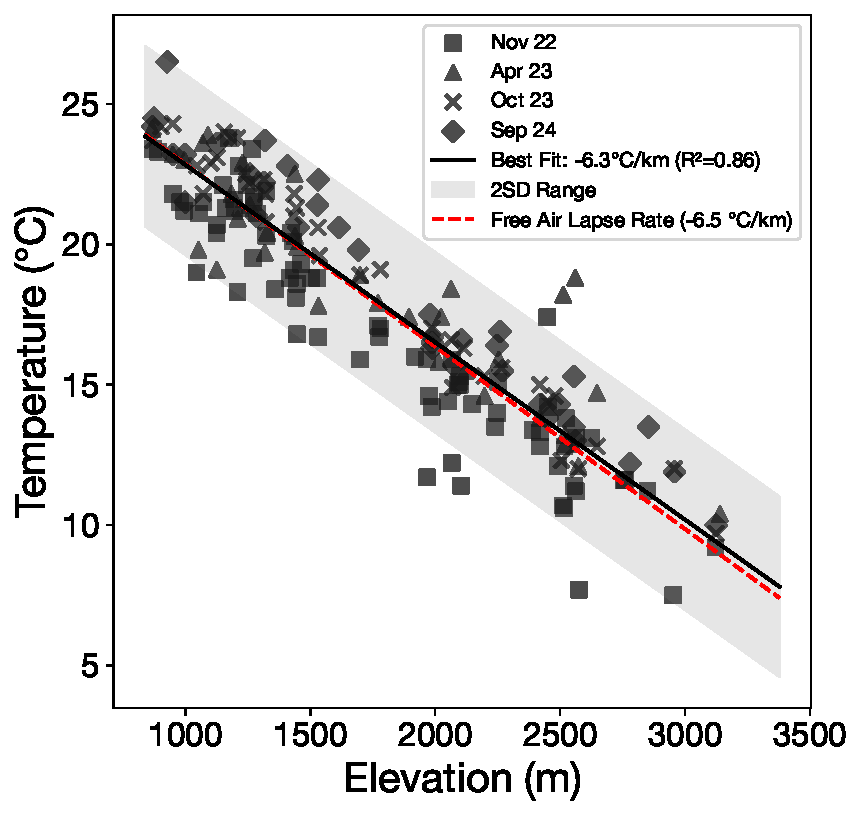
\includegraphics[width=0.7\textwidth]{Temperature_Elevation_Season.pdf}
    \caption{Temperature against elevation for each sampled season, with grey band representing two standard deviations from the mean. Lapse rate is consistent with the free air adiabatic lapse rate within error.}
    \label{fig:temperature}
\end{figure}

\FloatBarrier




% \begin{itemize}

% \item{What is the lat long extent of the study area?}

% 85.441 - 85.601 E, 27.822 - 28.157 N

% \item{What is the elevation range of the catchment?}

% 786 - 5697m

% \item{What is the area that the river drains? How do you calculate that (i.e. DEM)?}

% 325 km$^2$

% \item{What is the geology of the area?}



% \item{What is the climate of the area? what is it influenced by? i.e. monsoon, etc.}

% Bookhagen and Burbank (2010) identify two main climatic influences in the Himalayas: the monsoon system and the westerlies. The westerly winds, typical of this latitude, are responsible for the dry season in the Himalayas. The system is further divided into the East Asian and Indian Monsoon systems, which interact with each other. The high elevation of the High Himalayas creates a barrier that affects atmospheric circulation.  Bookhagen et al. (2005b) suggest that the Tibetan Plateau's high elevation generates a low-pressure cell near the surface, altering atmospheric circulation patterns.  This is one explanation for the monsoon, though other studies present differing views (see Bookhagen and Burbank, 2010 for a discussion). The source of precipitation during the Indian Summer Monsoon (ISM) affecting Melamchi is the Bay of Bengal, due to the strong pressure gradient that changes the westerly winds to southerly winds. This temperature gradient reverses in the winter, when the oceans are warm and the High Himalaya is cold.


% The high elevation of the High Himalayas creates a barrier that affects atmospheric circulation.  Bookhagen et al. (2005b) suggest that the Tibetan Plateau's high elevation generates a low-pressure cell near the surface, altering atmospheric circulation patterns.  This is one explanation for the monsoon, though other studies present differing views (see Bookhagen and Burbank, 2010 for a discussion). 


% Factor of 12 variation in runoff Tipper et al, 2006 and Sharma 1997


% \item{What is past literature on rainfall in monsoon season?}

% \item{What about clouds and fog? Especially when you are here?}

% \item{What are the annual mean temperatures at different elevations?}

% 24C at base elevation, ~900masl and 8C at highest elevation, ~3200masl.

% \item{What is the lapse rate like?}

% \item{What is the vegetation like?}

% Veget


% \item{Make sure to insert a description of the catchment: catchment, Area, mean slope, mean elevation, elevation range, land cover type, geology, Lat Long range}



% elevation range from DEM
% area from DEM, and software to figure out catchment area

% \end{itemize}